\documentclass{beamer}
%\usetheme{Madrid} % My favorite!
%\usetheme{Boadilla} % Pretty neat, soft color.
%\usetheme{default}
\usetheme{Warsaw}
%\usetheme{Bergen} % This template has nagivation on the left
%\usetheme{Frankfurt} % Similar to the default 
%with an extra region at the top.
\usecolortheme{seahorse} % Simple and clean template
%\usetheme{Darmstadt} % not so good
% Uncomment the following line if you want %
% page numbers and using Warsaw theme%
%\setbeamertemplate{footline}[page number]
\setbeamercovered{transparent}
%\setbeamercovered{invisible}
% To remove the navigation symbols from 
% the bottom of slides%
\setbeamertemplate{navigation symbols}{} 
\usepackage{epstopdf}
\usepackage{pgf}
\usepackage{tikz}
\usepackage{setspace} %Spacing
\usepackage{graphicx}
\usepackage{caption}
\usepackage{natbib}
\usepackage{wrapfig}
%\usepackage{subcaption}
\usepackage{enumerate}
\usetikzlibrary{positioning,shapes.geometric}
\usetikzlibrary{arrows}
\DeclareMathOperator*{\argmin}{arg\,min}

\usepackage{hyperref}
\hypersetup{
    colorlinks,
    citecolor=black,
    filecolor=black,
    linkcolor=blue,
    urlcolor=black
}


\newcommand{\Om}{\Omega}


\newcommand{\bs}[1]{\boldsymbol{#1}}
\newcommand{\wt}[1]{\widetilde{#1}}
\newcommand{\wh}[1]{\widehat{#1}}
\newcommand{\ol}[1]{\overline{#1}}
\newcommand{\e}{\varepsilon}
%\usepackage{bm}         % For typesetting bold math (not \mathbold)
%\logo{\includegraphics[height=0.6cm]{yourlogo.eps}}
%
\title[\texttt{Intro to Git}]{Introduction to Git}
\author[Asad Haris]{Asad Haris}
\institute[Dept of Biostatistics]
{Department of Biostatistics \\
University of Washington\\
\medskip
}
\date{\today}
% \today will show current date. 
% Alternatively, you can specify a date.
%
\begin{document}

\begin{frame}
\titlepage
\end{frame}

\section{Step 0}
\begin{frame}
\frametitle{Step 0: Installation}
\begin{itemize}
\item \textbf{Install Git}: \url{https://git-scm.com/downloads}
\item \textbf{Easy Install for Linux}
\begin{itemize}
\item \texttt{apt-get install git} (Ubuntu/Debian)
\item \texttt{yum install git} (Fedora)
\item Others can be found at \url{https://git-scm.com/download/linux}
\end{itemize}

\item This is all we need to get started. You can work with Git completely off-line. 
%If you wish to follow this tutorial to the end, 

\pause
\item Make an account at 

\url{https://github.com/} or \url{https://bitbucket.org/} 

We will discuss differences between the two. 
\end{itemize}



\end{frame}

\section{Introduction}

\begin{frame}
\centering
\Large While everything is downloading/installing... 
\end{frame}

\begin{frame}
\frametitle{What is Git?}
\begin{itemize}
\item Git is a version control system
\item As the name suggests, a system to manage different versions of a project
\item A project in Git is called a repository/repo 
\item Git allows us to take it a step further with many other features
\item Collaborating on a project is much simpler with Github/Bitbucket
\end{itemize}
\end{frame}

\begin{frame}
\centering
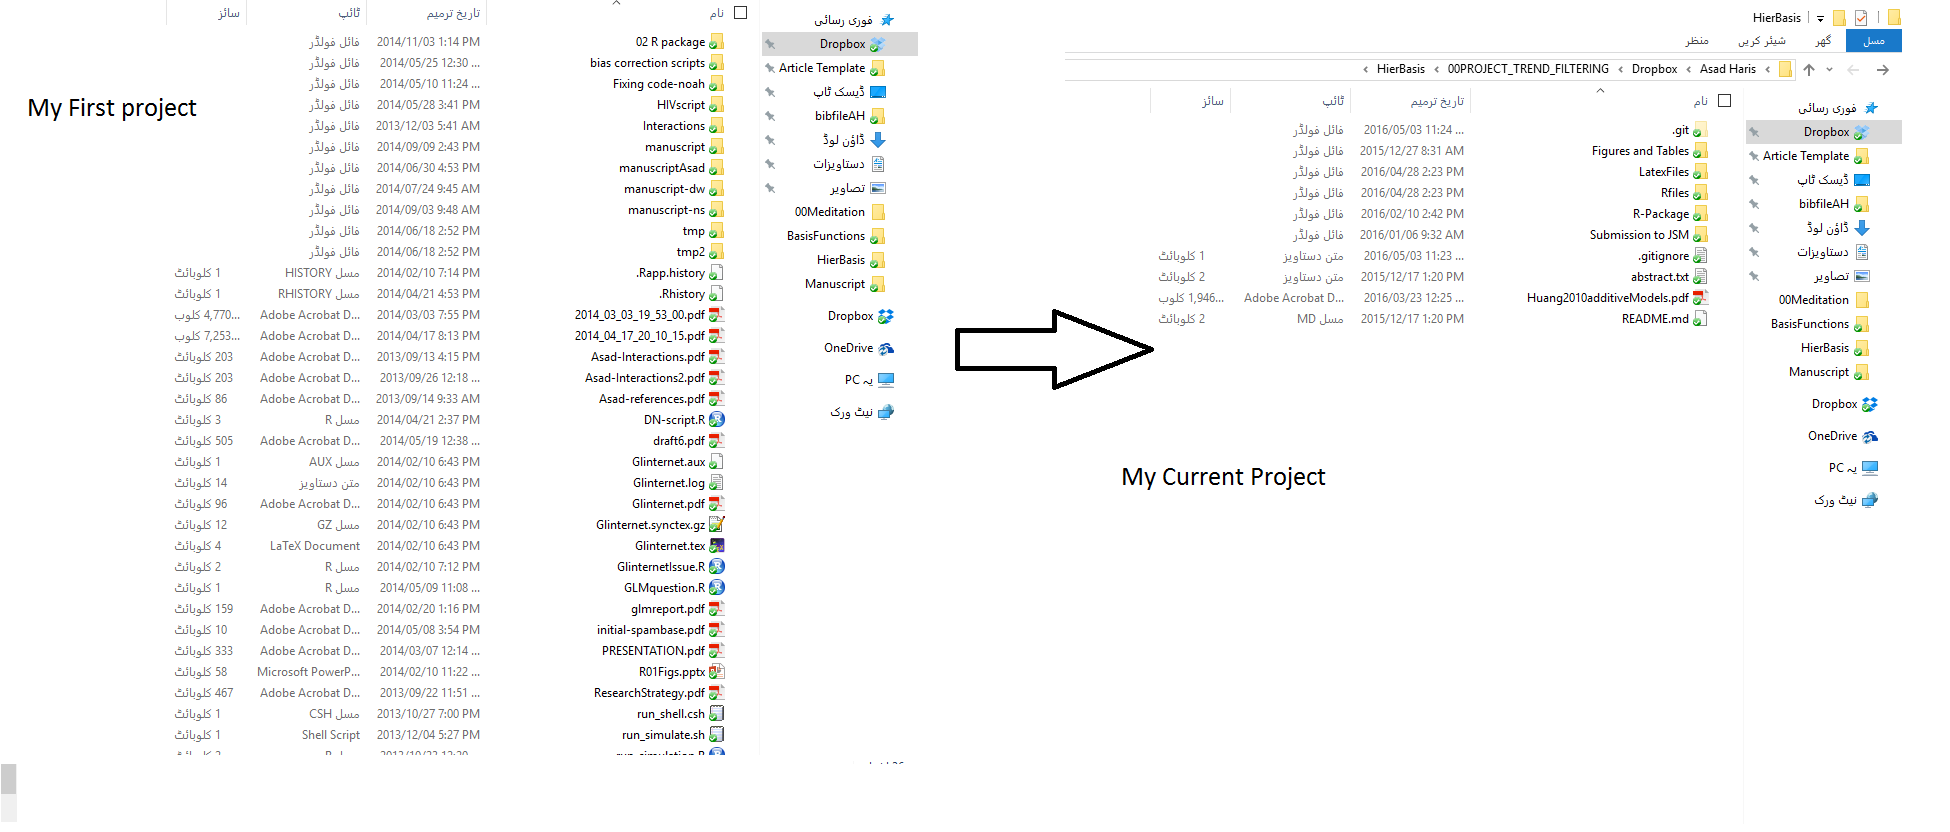
\includegraphics[scale = 0.25]{history}
\end{frame}


\begin{frame}
\frametitle{How does git work?}
\centering
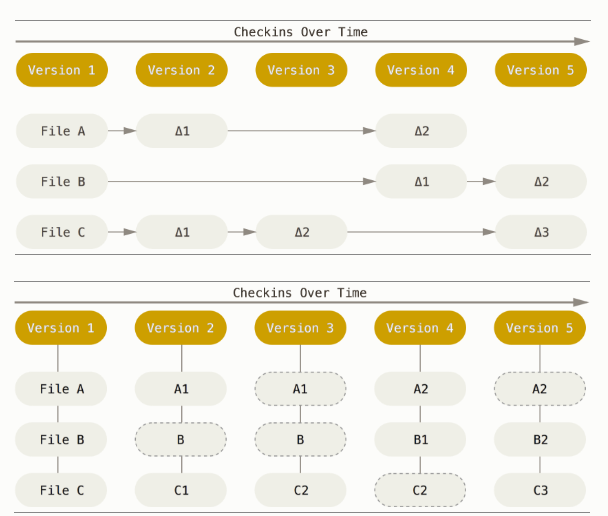
\includegraphics[scale = 0.5]{workflow}
\end{frame}

\begin{frame}
\frametitle{So why Git?}
\textbf{Advantages}
\begin{itemize}
\item Allows you manage different versions of your project
\item We can go back in time to previous versions 
\item Isn't restricted to specific type of projects (not just for computer scientists)
\item Makes collaboration on a project really easy
\item We have nice tools like GitHub and Bitbucket for collaboration and online sharing
\end{itemize}

\textbf{Disadvantages}
\begin{itemize}
\item Initial learning curve, which we will overcome today
\end{itemize}
\end{frame}


\begin{frame}
\frametitle{As promised Github vs. Bitbucket}
Essentially, Github/Bitbucket is a remote location to store/share your repositories


\begin{table}
\centering

\begin{tabular}{c|cc}
\hline
 & Github & Bitbucket\\
\hline
Cost & Free & Free\\
Public Repositories & Unlimited & Unlimited\\
Private Repositories & 5\footnote[1] & Unlimited\\
Collaborators & Unlimited & 5\footnote[2] \\
\end{tabular}
\caption{1. After student discount. 2. For the free account, can have upto unlimited collaborators with paid account.}
\end{table}

\end{frame}



\section{Main Tutorial}

\begin{frame}
\centering
\Large Working with Git
\end{frame}

\begin{frame}[fragile]
\frametitle{First Steps: Configure Git}
Once Git is installed, we begin with configuring Git. 

\begin{verbatim}
git config --global user.name "asadharis"
git config --global user.email aharis@uw.edu
git config --global color.ui true
\end{verbatim}

This only needs to be done once!
\end{frame}

\begin{frame}
\frametitle{Outline of Project}
We will consider a simple project: A mini version of an assignment
\begin{enumerate}[1.]
\item We will first \textit{initialize} a git repo
\item Begin writing up the assignment
\item Make an Rfile for all our work in R
\item Upload our Repo to github and collaborating
\end{enumerate} 
\end{frame}

\begin{frame}[fragile]
\frametitle{Starting a repo is easy}
Starting a git Repo is very simple
\begin{verbatim}
# Make a dir where we want our project to reside
mkdir hw1_stat101 
# Move to the working directory
cd hw1_stat101

# Initialize a Git repo
git init   # Really this is it!

# Check to see what the command did
ls -l -a   # Should see the .git folder
\end{verbatim}
\end{frame}


\begin{frame}[fragile]
\frametitle{Begin work on the project}
\begin{verbatim}
mkdir latex_files r_files
cd latex_files

vim hw1.tex
... Latex text goes here ...

pdflatex hw1.tex
\end{verbatim}
\end{frame}


\begin{frame}[fragile]
\frametitle{The first commit}
Making a new commit is as easy as 
\begin{verbatim}
git status
git add --all
git commit -m "My first commit"
\end{verbatim}

\centering
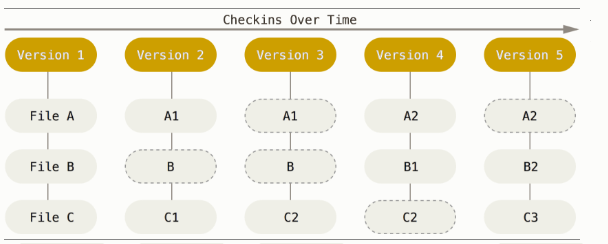
\includegraphics[scale = 0.4]{workflowRecall}


\end{frame}


\begin{frame}
\frametitle{Some details about commiting}
\centering
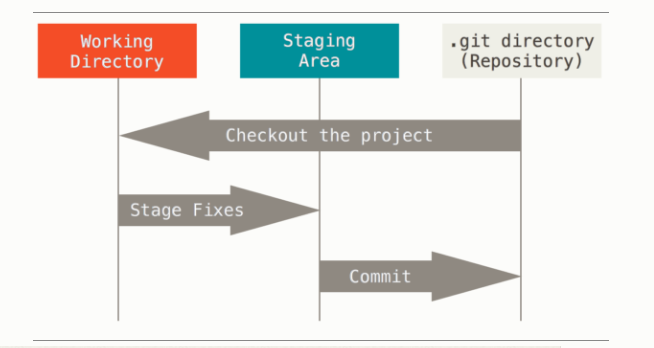
\includegraphics[scale = 0.6]{commitWorkflow}
\end{frame}


\begin{frame}[fragile]
\frametitle{Adding an R file and Git history}
We can now add an Rfile, run our simulations and make another commit.


After this we now see the history of our project using the \texttt{log} command

\begin{verbatim}
git log  # Basic view

git log --help  # View other options

git log --graph   # The one I like
\end{verbatim}
\end{frame}

\begin{frame}
\frametitle{Working online: Sign-in to Github}
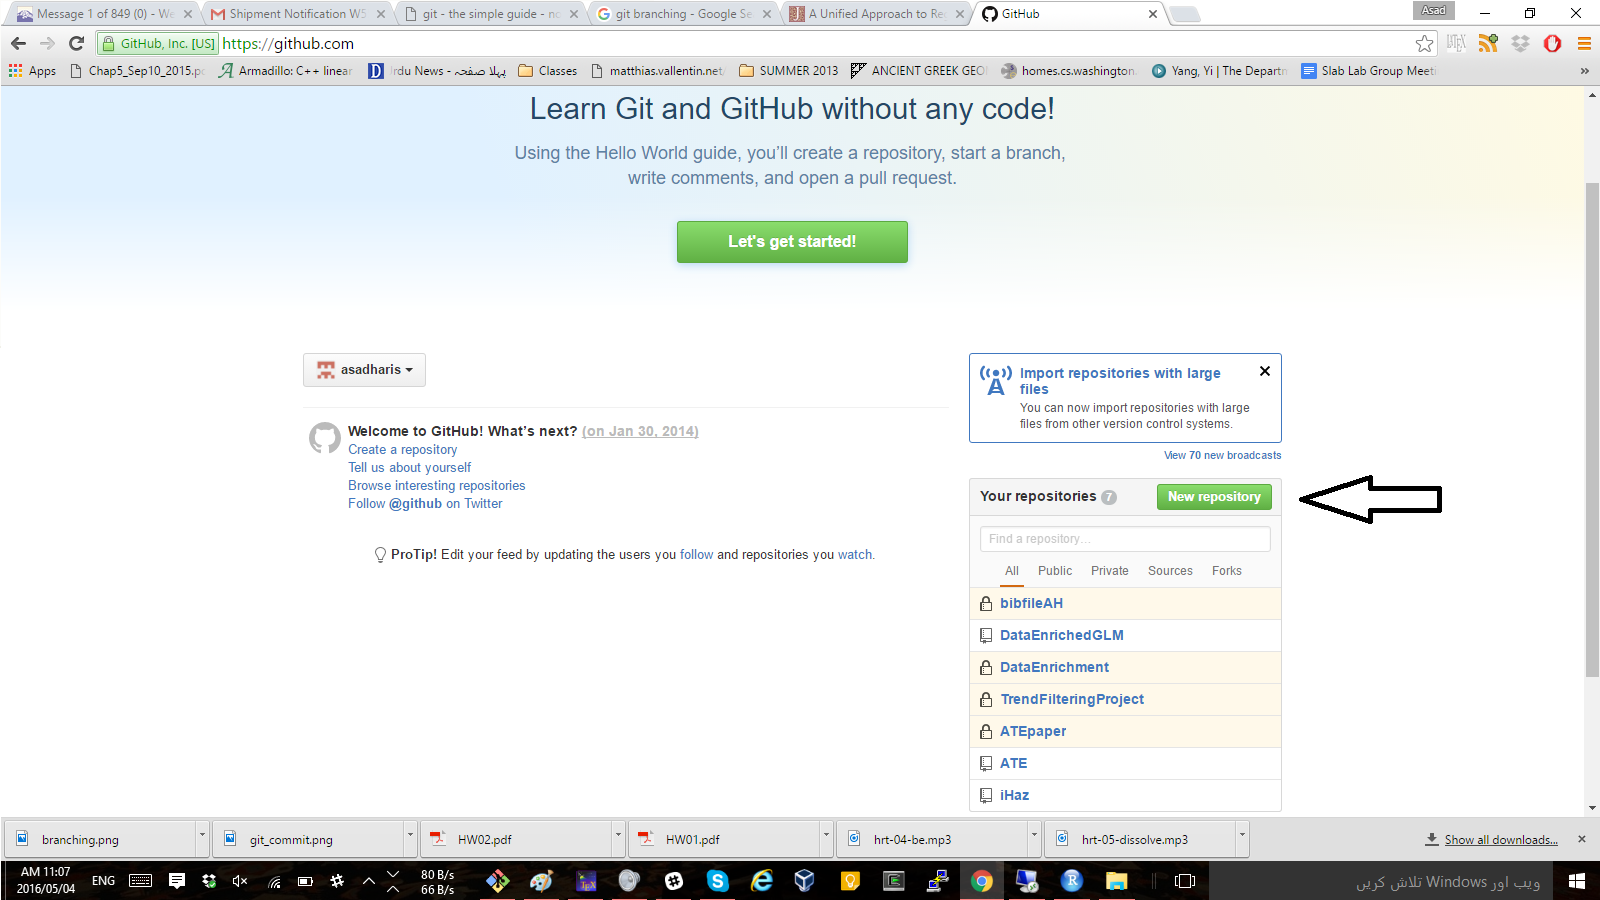
\includegraphics[scale = 0.3]{signin}
\end{frame}

\begin{frame}
\centering
\frametitle{Working online: Make the Repo}
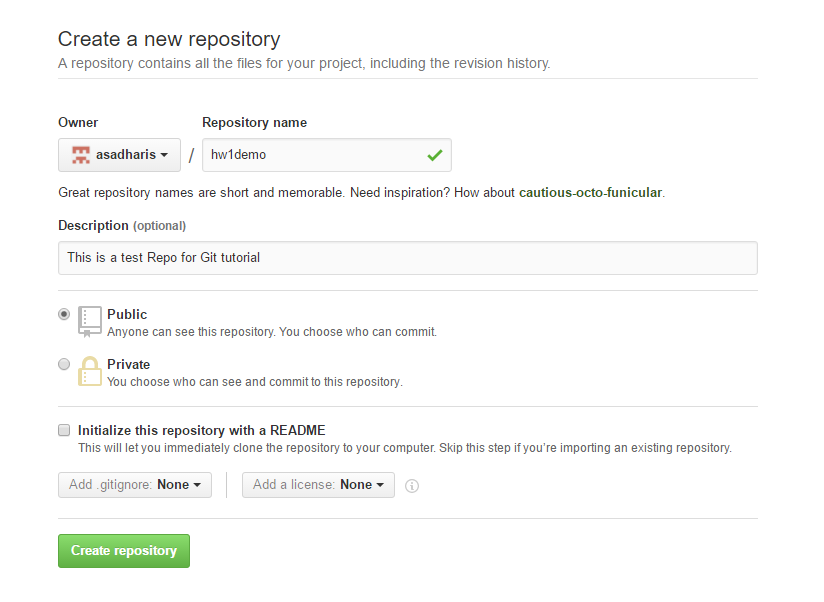
\includegraphics[scale = 0.4]{makerepo}
\end{frame}

\begin{frame}
\centering
\frametitle{Working online: we will use option 2}
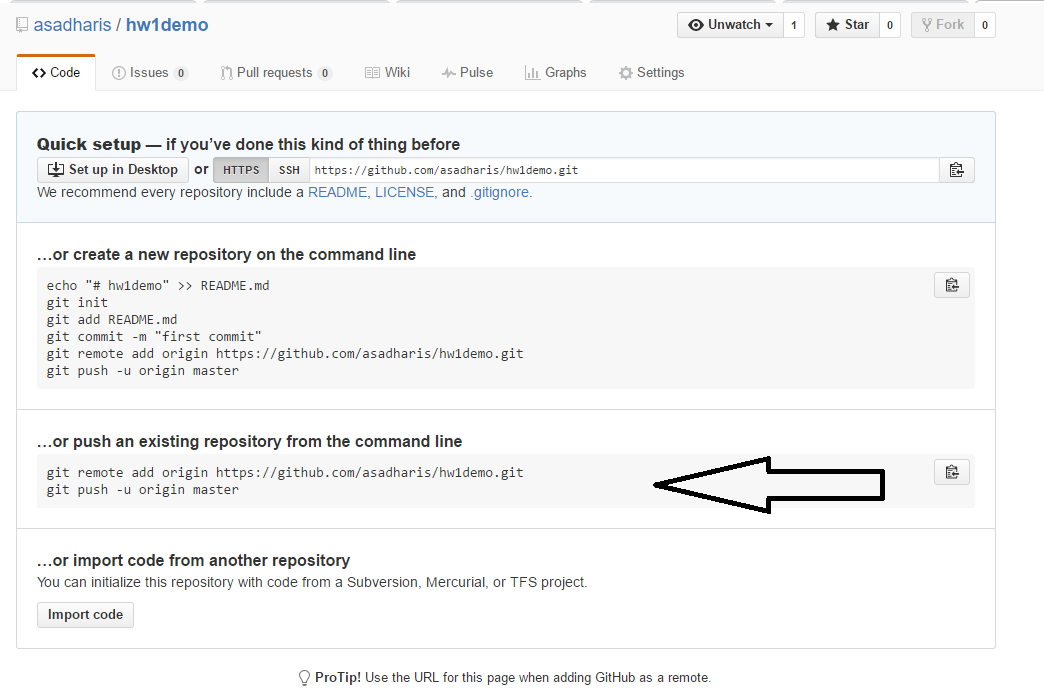
\includegraphics[scale = 0.37]{makerepo2}
\end{frame}


\begin{frame}[fragile]
\frametitle{Possible issue}
The instructions on github may not work for linux/mac. So try the following 
\begin{verbatim}
git remote set-url origin \\
	 https://github.com/asadharis/hw1demo.git
\end{verbatim}
\end{frame}


\begin{frame}[fragile]
\frametitle{Collaborating }
Say your collaborator made changes to project and you begin work the next day.

First you need to bring in all the changes they made. For this we have the pull command
\begin{verbatim}
git pull
\end{verbatim}

\pause

\textbf{Working in Git is really just these 5 commands}
\begin{tabular}{c|c}
\hline
\texttt{pull} & Pulls down current version of repo\\
\hline
\texttt{status} & check status of repo\\
\texttt{add} & add files to staging area\\
\texttt{commit} & commit staged files\\
\hline
\texttt{push} & Pushes files to Remote\\
\hline
\end{tabular}
\end{frame}


\begin{frame}[fragile]
\frametitle{Review what we have done}
A short summary of what we have done so far
\begin{verbatim}
git init  # Start a repo/begin work
git status  # Check status of changes made
git add  --all # Stage all the files
git commit -m "Some message"   # A version is complete

# Set-up remote and then
git push
git pull

# Check progress of project
git log
\end{verbatim}
\end{frame}


\section{Other Features}


\begin{frame}[fragile]
\frametitle{Going back in Time}
We have two options 

1. \textbf{Review history/old versions}
\begin{verbatim}
git checkout [commit-number] 
\end{verbatim}

2. \textbf{Go back in time or start over}
\begin{verbatim}
git reset [commit-number]  # Keep local changes
git reset [commit-number] --hard  # Destroy local changes
\end{verbatim}
\end{frame}

\begin{frame}
\frametitle{Merge Conflict}
If two people are working on the same file we may have some conflicts.

See terminal
\end{frame}

\begin{frame}
\frametitle{Branching}
\centering
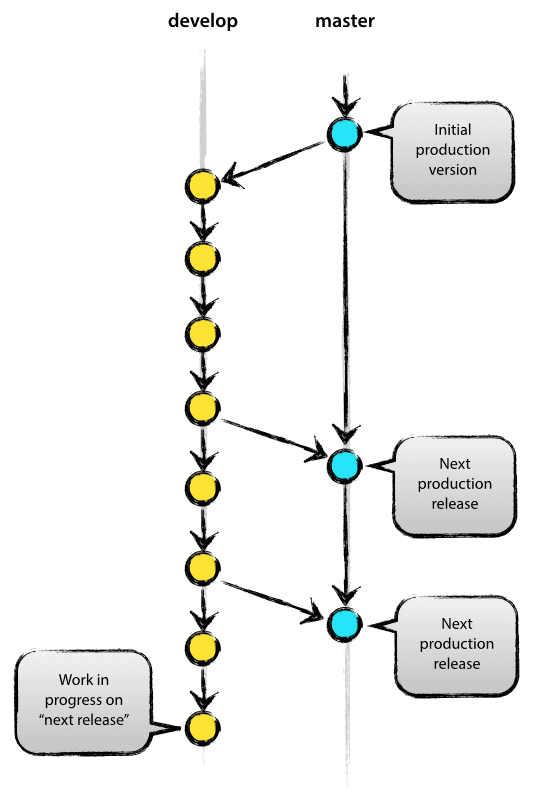
\includegraphics[scale = 0.25]{branching}
\end{frame}

\begin{frame}[fragile]
\frametitle{Branching}

For working with branches we have the following commands
\begin{verbatim}
git branch  # View all branches
git branch testV2  # Make a new branch
git checkout testV2  # Move to other branch 
\end{verbatim}

\end{frame}


\begin{frame}
\frametitle{The .gitignore file}
\begin{itemize}
\item There may be some files we don't want to track
\item In some cases it is good practice to not track some files. e.g. the extra files latex generates will always lead to merge conflicts
\item Add all untracked files in a text file called: .gitignore
\item I usually borrow a gitignore file and add things to it. e.g. 
\url{https://gist.github.com/kogakure/149016}
\end{itemize}
\end{frame}

\begin{frame}
\frametitle{Conclusion}
\begin{itemize}
\item Git can be used for projects of all sizes
\item Other useful things can be done with a bit of creativity
\item Many tutorials out there: 
\begin{itemize}
\item (Official) \url{https://git-scm.com/docs/gittutorial} 
\item (More detailed) \url{https://www.atlassian.com/git/tutorials/}
\item (My favorite) \url{https://www.youtube.com/watch?v=0fKg7e37bQE}
\end{itemize}
\item A cheat-sheet I use \url{https://training.github.com/kit/downloads/github-git-cheat-sheet.pdf}
\item As always google is your friend
\end{itemize}
\end{frame}





\end{document} 